\documentclass[12pt,a4paper]{article}
\usepackage[utf8]{vietnam}
\usepackage{amsmath,amssymb}
\usepackage{tabularx}
\usepackage{tikz}
\usetikzlibrary{calc,angles,quotes,arrows.meta,patterns}
\usepackage{xcolor}
\usepackage{enumitem}
\usepackage{fancyhdr}
\usepackage[top=1.2cm, bottom=1.2cm, left=1.5cm, right=1.5cm]{geometry}
\usepackage[dethi]{ex_test}
\SAOPTN{widthSA=2.6,heightSA=0.62}

\setlength{\headheight}{15pt}
\setlength{\parskip}{0pt}

\pagestyle{fancy}
\fancyhf{}
\rhead{\textit{Môn Toán 6 -- Đề số 9}}
\lhead{\textit{Bộ đề ôn tập Giữa học kì I}}
\cfoot{\thepage}

\begin{document}

% --- KHUNG TIÊU ĐỀ ĐỀ THI ---
\noindent
\begin{tabularx}{\linewidth}{X r}
\textbf{TRƯỜNG THCS: \dotfill} & \textbf{ĐỀ KIỂM TRA ĐỊNH KỲ GIỮA HỌC KỲ I} \\
\textbf{Họ và tên: \dotfill} & \textbf{NĂM HỌC 2026 -- 2027} \\
\textbf{Lớp: \dotfill \quad SBD: \dotfill} & \textbf{Môn: TOÁN 6} \\
\hline
\end{tabularx}
\vspace{2mm}

\begin{center}
  \textbf{\large ĐỀ ÔN TẬP GIỮA HỌC KỲ I -- ĐỀ SỐ 9}\\
  \textit{Thời gian làm bài: 90 phút (Không kể thời gian phát đề)}
\end{center}
\vspace{1mm}

% --- PHẦN I ---
\noindent\textbf{\large PHẦN I. CÂU TRẮC NGHIỆM NHIỀU PHƯƠNG ÁN LỰA CHỌN (3,0 điểm)}

\textit{Thí sinh trả lời từ câu 1 đến câu 12. Mỗi câu hỏi thí sinh chỉ chọn một phương án duy nhất.}

\vspace{1mm}
\begin{ex}
Cho tập hợp $M = \{1; 5; a; b\}$. Trong các khẳng định sau, khẳng định sai là:
\choice
{$1 \in M$}
{$c \notin M$}
{$a \in M$}
{\True $b \notin M$}
\end{ex}

\begin{ex}
Tập hợp $P$ các số tự nhiên lớn hơn 9 có thể viết là:
\choice
{$P = \{x \in \mathbb{N} \mid x < 10\}$}
{$P = \{x \in \mathbb{N} \mid x \le 10\}$}
{$P = \{x \in \mathbb{N} \mid x > 10\}$}
{\True $P = \{x \in \mathbb{N} \mid x \ge 10\}$}
\end{ex}

\begin{ex}
Số liền trước và số liền sau của số $2\,024$ lần lượt là:
\choice
{$2\,023; 2\,024$}
{$2\,022; 2\,023$}
{$2\,026; 2\,026$}
{\True $2\,023; 2\,025$}
\end{ex}

\begin{ex}
Với $a, m, n$ là các số tự nhiên ($a \ne 0$), khẳng định nào sau đây đúng?
\choice
{\True $a^m \cdot a^n = a^{m+n}$}
{$a^m \cdot a^n = a^{m-n}$}
{$a^m \cdot a^n = a^{m \cdot n}$}
{$a^m \cdot a^n = (a \cdot m) + n$}
\end{ex}

\begin{ex}
Trong các số $0; 1; 2; 4; 6; 16$, số nào là bội của 8?
\choice
{$1; 2; 4$}
{$2; 4$}
{$0; 1; 16$}
{\True $0; 16$}
\end{ex}

\begin{ex}
Hình vuông có cạnh bằng $15\text{ cm}$ thì chu vi bằng:
\choice
{$225\text{ cm}^2$}
{$225\text{ cm}$}
{$60\text{ cm}^2$}
{\True $60\text{ cm}$}
\end{ex}

\begin{ex}
Tập hợp các ước chung của 9 và 15 là:
\choice
{\True $\{1; 3\}$}
{$\{0; 3\}$}
{$\{1; 5\}$}
{$\{1; 3; 9\}$}
\end{ex}

\begin{ex}
Trong các số sau đây, số nào chia hết cho $2^3$?
\choice
{$23$}
{$3^5$}
{\True $4^2$}
{$6^2$}
\end{ex}

\begin{ex}
Cho tam giác $ABC$ đều. Khẳng định nào sau đây là sai?
\choice
{Ba cạnh bằng nhau: $AB = BC = CA$}
{\True Ba đỉnh $A, B, C$ bằng nhau}
{Ba góc ở đỉnh $A, B, C$ bằng nhau}
{Ba góc $\widehat{A}, \widehat{B}, \widehat{C}$ bằng nhau}
\end{ex}

\begin{ex}
Cho tam giác đều $ABC$ có cạnh $AB = 3\text{ cm}$. Chu vi của tam giác đều $ABC$ là:
\choice
{$3\text{ cm}$}
{\True $9\text{ cm}$}
{$12\text{ cm}$}
{$18\text{ cm}$}
\end{ex}

\begin{ex}
Mảnh đất hình thang vuông $ABCD$ như hình vẽ, biết $AB = 12\text{ m}$, $DC = 26\text{ m}$, diện tích hình chữ nhật $ABKD$ là $168\text{ m}^2$. Diện tích mảnh đất hình thang $ABCD$ là:
\begin{center}
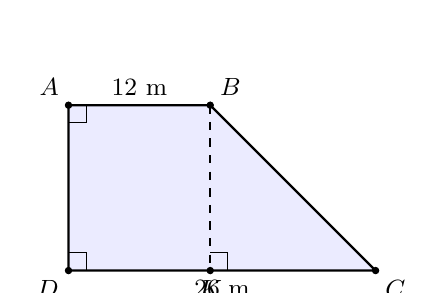
\begin{tikzpicture}[scale=0.75, font=\small]
  \coordinate (D) at (0,0);
  \coordinate (K) at (2.4,0);
  \coordinate (C) at (5.2,0);
  \coordinate (B) at (2.4,2.8);
  \coordinate (A) at (0,2.8);
  \draw[thick, fill=blue!8] (A) -- (B) -- (C) -- (D) -- cycle;
  \draw[thick, dashed] (B) -- (K);
  \draw (0,0.3) -- (0.3,0.3) -- (0.3,0);
  \draw (0,2.5) -- (0.3,2.5) -- (0.3,2.8);
  \draw (2.4,0.3) -- (2.7,0.3) -- (2.7,0);
  \filldraw (A) circle (1.5pt) node[above left] {$A$};
  \filldraw (B) circle (1.5pt) node[above right] {$B$};
  \filldraw (C) circle (1.5pt) node[below right] {$C$};
  \filldraw (D) circle (1.5pt) node[below left] {$D$};
  \filldraw (K) circle (1.5pt) node[below] {$K$};
  \node[above] at (1.2,2.8) {$12\text{ m}$};
  \node[below] at (2.6,0) {$26\text{ m}$};
\end{tikzpicture}
\end{center}
\choice
{$168\text{ m}^2$}
{$133\text{ m}^2$}
{\True $266\text{ m}^2$}
{$312\text{ m}^2$}
\end{ex}

\begin{ex}
Bạn An có ngày sinh là số nguyên tố lớn nhất nhỏ hơn 20, tháng sinh của bạn là số nguyên tố nhỏ nhất. Vậy bạn An có ngày và tháng sinh là:
\choice
{Ngày 19 tháng 3}
{\True Ngày 19 tháng 2}
{Ngày 7 tháng 2}
{Ngày 7 tháng 3}
\end{ex}


\vspace{1mm}
\noindent\textbf{BẢNG TRẢ LỜI TRẮC NGHIỆM PHẦN I:}
\begin{center}
\begin{tabular}{|c|c|c|c|c|c|c|c|c|c|c|c|c|}
\hline
\textbf{Câu} & \textbf{1} & \textbf{2} & \textbf{3} & \textbf{4} & \textbf{5} & \textbf{6} & \textbf{7} & \textbf{8} & \textbf{9} & \textbf{10} & \textbf{11} & \textbf{12} \\
\hline
\textbf{Chọn} & \rule{0pt}{0.65cm} & & & & & & & & & & & \\
\hline
\end{tabular}
\end{center}
\vspace{2mm}

\setcounter{ex}{0}
\noindent\textbf{\large PHẦN II. CÂU TRẮC NGHIỆM ĐÚNG SAI (2,0 điểm)}

\textit{Thí sinh trả lời câu 1 và câu 2. Trong mỗi ý a), b), c), d) ở mỗi câu, thí sinh chọn đúng hoặc sai.}

\vspace{1mm}
\begin{ex}
Xét tính đúng/sai của các mệnh đề sau:
\choiceTF
{\True Số $1975$ là hợp số}
{Mọi số nguyên tố đều là số lẻ}
{\True Số 1 không là hợp số cũng không là số nguyên tố}
{Tổng của hai số nguyên tố bất kì luôn là một số chẵn}
\end{ex}

\begin{ex}
Cho hình thoi $MNPQ$ có độ dài hai đường chéo lần lượt là $MP = 10\text{ cm}$ và $NQ = 6\text{ cm}$. Xét tính đúng/sai của các khẳng định sau:
\choiceTF
{\True Bốn cạnh $MN, NP, PQ, QM$ có độ dài bằng nhau}
{Hai đường chéo $MP$ và $NQ$ song song với nhau}
{\True Diện tích của hình thoi $MNPQ$ là $30\text{ cm}^2$}
{\True Hai đường chéo $MP$ và $NQ$ cắt nhau tại trung điểm của mỗi đường và vuông góc với nhau}
\end{ex}


\noindent\textbf{BẢNG TRẢ LỜI PHẦN II:}
\begin{center}
\begin{tabular}{|c|c|c|c|c||c|c|c|c|c|}
\hline
\textbf{Câu 1} & \textbf{a)} & \textbf{b)} & \textbf{c)} & \textbf{d)} & \textbf{Câu 2} & \textbf{a)} & \textbf{b)} & \textbf{c)} & \textbf{d)} \\
\hline
\textbf{Đ/S} & \rule{0pt}{0.6cm} & & & & \textbf{Đ/S} & & & & \\
\hline
\end{tabular}
\end{center}
\vspace{2mm}

\setcounter{ex}{0}
\noindent\textbf{\large PHẦN III. CÂU HỎI TRẢ LỜI NGẮN (2,0 điểm)}

\textit{Thí sinh trả lời câu 1 và câu 2. Điền kết quả số vào ô trống tương ứng.}

\vspace{1mm}
\begin{ex}
Tìm số tự nhiên $x$ thỏa mãn $3 \cdot (x - 5) = 2^3 \cdot 3$. \shortans{13}
\end{ex}

\begin{ex}
Một hình bình hành có độ dài một cạnh bằng $10\text{ cm}$ và chiều cao tương ứng bằng $6\text{ cm}$. Tính diện tích của hình bình hành đó (theo đơn vị $\text{cm}^2$). \shortans{60}
\end{ex}


\setcounter{ex}{0}
\noindent\textbf{\large PHẦN IV. TỰ LUẬN (3,0 điểm)}

\textit{Thí sinh trình bày chi tiết lời giải vào giấy làm bài.}

\vspace{1mm}
\begin{ex} (0,75 điểm)
Viết tập hợp $A$ các số tự nhiên lớn hơn 9 và nhỏ hơn 15 bằng hai cách.
\end{ex}
\vspace{1.5mm}

\begin{ex} (1,0 điểm)
Thực hiện phép tính:
\begin{enumerate}[label=\textbf{\alph*)}, leftmargin=0.8cm, itemsep=2pt]
\item (0,5 điểm) $(30 - 10 \cdot 2) : 5$
\item (0,5 điểm) $135 \cdot 3^2 - 3^2 \cdot 130$
\end{enumerate}
\end{ex}
\vspace{1.5mm}

\begin{ex} (0,75 điểm)
Một mảnh vườn hình chữ nhật có chiều dài $40\text{ m}$ và chiều rộng $30\text{ m}$.
\begin{enumerate}[label=\textbf{\alph*)}, leftmargin=0.8cm, itemsep=2pt]
\item (0,375 điểm) Tính chu vi và diện tích của mảnh vườn.
\item (0,375 điểm) Biết rằng mỗi túi hạt giống gieo vừa đủ $100\text{ m}^2$ đất và mỗi túi giá $40\,000$ đồng. Hỏi cần bao nhiêu túi hạt giống để gieo vừa hết mảnh vườn và cần bao nhiêu tiền?
\end{enumerate}
\end{ex}
\vspace{1.5mm}

\begin{ex} (0,5 điểm)
Cho các số tự nhiên: $23; 87; 64; 270; 425; 136; 2808$.
\begin{enumerate}[label=\textbf{\alph*)}, leftmargin=0.8cm, itemsep=2pt]
\item (0,125 điểm) Số nào chia hết cho 2?
\item (0,125 điểm) Số nào chia hết cho 3?
\item (0,125 điểm) Số nào chia hết cho 5?
\item (0,125 điểm) Số nào chia hết cho cả 2 và 5?
\end{enumerate}
\end{ex}
\vspace{1.5mm}


\begin{center}
\rule{4cm}{0.4pt}\\
\textit{--- HẾT ---}
\end{center}
\end{document}
